\documentclass[10pt]{standalone}
\usepackage[utf8]{inputenc}
\usepackage{pgf,tikz,pgfplots}
\pgfplotsset{compat=1.15}
\usepackage{mathrsfs}
\usetikzlibrary{arrows}
\pagestyle{empty}
\begin{document}

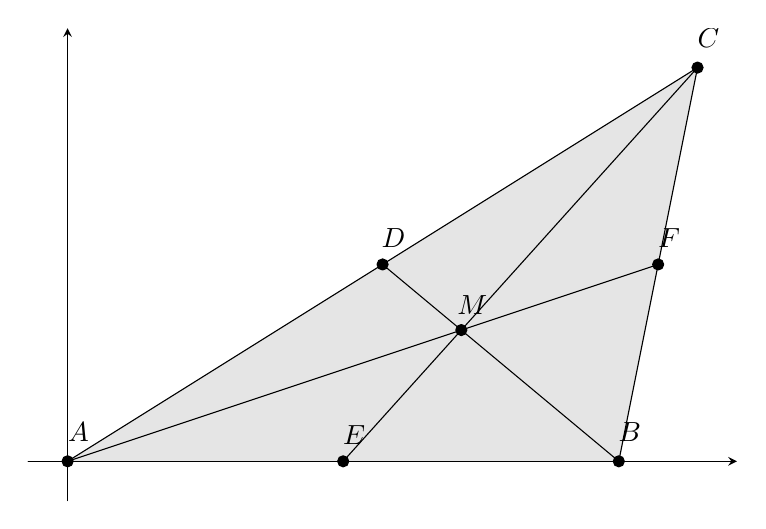
\begin{tikzpicture}[line cap=round,line join=round,>=triangle 45,x=1.0cm,y=1.0cm]
\begin{axis}[
x=1.0cm,y=1.0cm,
axis lines=middle,
xmin=-0.5,
xmax=8.5,
ymin=-0.5,
ymax=5.5,
ticks=none,
]
\clip(-0.5,-0.5) rectangle (8.5,5.5);
\fill[,color=black,fill=black,fill opacity=0.1] (0.,0.) -- (7.,0.) -- (8.,5.) -- cycle;
\draw  (0.,0.)-- (7.,0.);
\draw  (7.,0.)-- (8.,5.);
\draw  (8.,5.)-- (0.,0.);
\draw  (0.,0.)-- (7.5,2.5);
\draw (7.,0.)-- (4.,2.5);
\draw (3.5,0.)-- (8.,5.);
\begin{scriptsize}
\draw [fill=black] (0.,0.) circle (2.0pt);
\draw[color=black] (0.14,0.37) node {$A$};
\draw [fill=black] (7.,0.) circle (2.0pt);
\draw[color=black] (7.14,0.37) node {$B$};
\draw [fill=black] (8.,5.) circle (2.0pt);
\draw[color=black] (8.14,5.37) node {$C$};

\draw [fill=black] (4.,2.5) circle (2.0pt);
\draw[color=black] (4.14,2.83) node {$D$};
\draw [fill=black] (3.5,0.) circle (2.0pt);
\draw[color=black] (3.64,0.33) node {$E$};
\draw [fill=black] (7.5,2.5) circle (2.0pt);
\draw[color=black] (7.64,2.83) node {$F$};

\draw [fill=black] (5.,1.6666666666666667) circle (2.0pt);
\draw[color=black] (5.14,1.99) node {$M$};
\end{scriptsize}
\end{axis}
\end{tikzpicture}
\end{document}